\begin{table}[!h]
\centering
\renewcommand{\arraystretch}{1}
\begin{tabular}[t]{|p{3.5cm}|p{10.5cm}|}	
	\hline
	\textbf{Strategy name} & {\sc Independent Multi-Walk}\\
	\hline
	\textbf{Cooperative} & 
	\begin{tabular}[t]{@{}l@{}}
	$\square$ Yes\\
	$\text{\rlap{$\checkmark$}}\square$ No
	\end{tabular}\\
	\hline
	\textbf{Description} & Same solver structure in the \soset{}.\\
	\hline
	\textbf{Topology} & 
	\begin{tabular}[t]{@{}l@{}}
	$\vardiamond$ Unconnected (See Figure~\ref{figtop:nc})
	\end{tabular}\\
	\hline 	
	{\bf Benchmarks} & 
	\begin{tabular}[t]{@{}l@{}}
		\sgp\\ \nqp\\ \carrp\\ \grp\\
	\end{tabular}\\
	\hline	
\end{tabular}
%\caption{\sgp}
\label{tab_resume:nocomm}
\end{table}

%\begin{minipage}{0.5\textwidth}
%\centering
%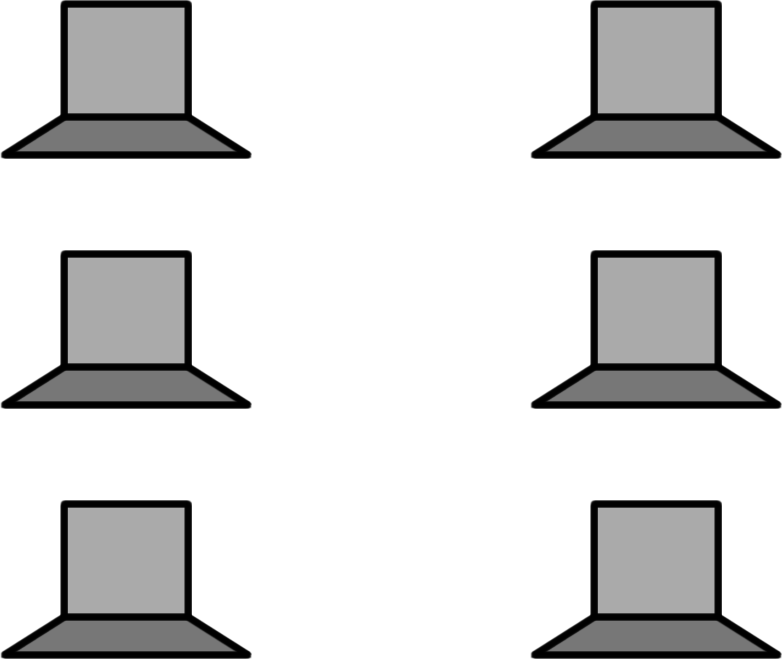
\includegraphics[width=0.5\linewidth]{no_conn.png}
%\captionof{figure}{Unconnected}\label{figtop:nc}
%\end{minipage}
%\begin{minipage}{0.5\textwidth}
%\centering
%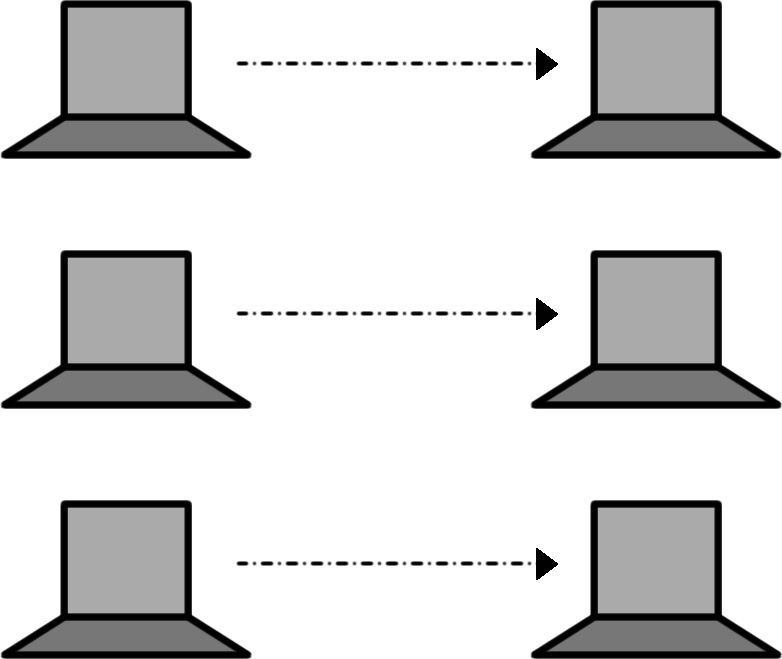
\includegraphics[width=0.5\linewidth]{1-1.png}
%\captionof{figure}{Point to point}\label{figtop:1-1}
%\end{minipage}

\begin{figure}[!h]
  \begin{minipage}[b]{0.5\textwidth}
    \centering
    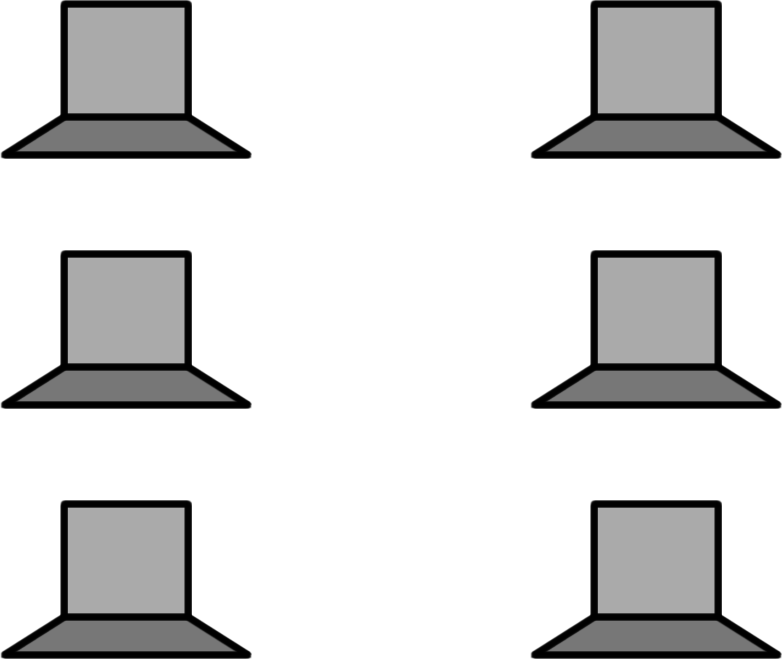
\includegraphics[width=0.6\textwidth]{no_conn.png}
    \caption{Unconnected}\label{figtop:nc}
  \end{minipage}
  \hfill
  \begin{minipage}[b]{0.5\textwidth}
  \centering
    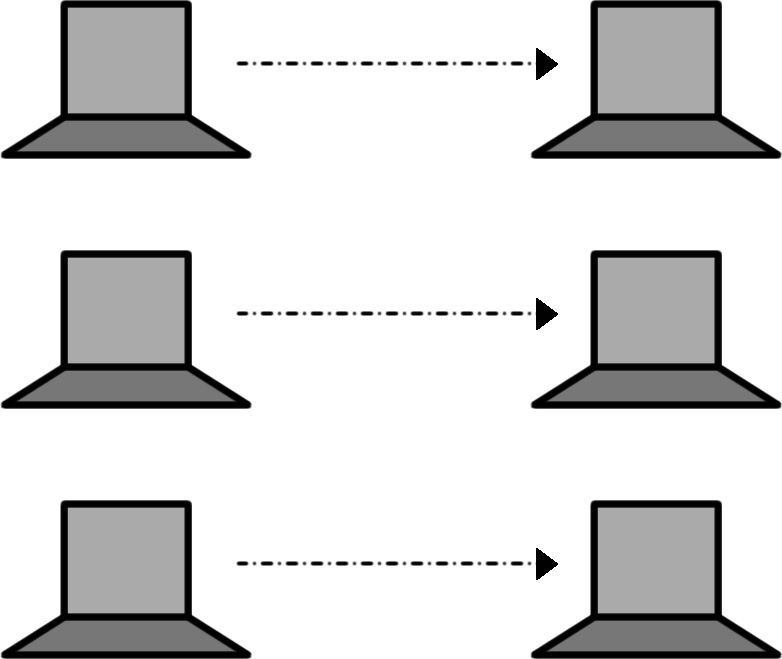
\includegraphics[width=0.6\textwidth]{1-1.png}
    \caption{Point to point}\label{figtop:1-1}
  \end{minipage}
\end{figure}

\begin{table}[!h]
\centering
\renewcommand{\arraystretch}{1}
\begin{tabular}[t]{|p{3.5cm}|p{10.5cm}|}
	\hline
	\textbf{Strategy name} & {\sc Simple Communication Strategy} (variant A)\\
	\hline
	\textbf{Cooperative} & 
	\begin{tabular}[t]{@{}l@{}}
	$\text{\rlap{$\checkmark$}}\square$ Yes\\
	$\square$ No
	\end{tabular}\\
	\hline
	\textbf{Description} & Same solver structure in the \soset{}. Communication in one sense of the current configuration, performed while applying the acceptance criterion of the new configuration for the next iteration.\\
	\hline
	\textbf{Topologies} & 
	\begin{tabular}[t]{@{}l@{}}
	$\vardiamond$ Point to point (See Figure~\ref{figtop:1-1})\\
	$\vardiamond$ Mixed point to point (See Figure~\ref{figtop:mix_1-1})\\
	$\vardiamond$ Bipartition (See Figure~\ref{figtop:1-n})\\
	$\vardiamond$ Mixed bipartition (See Figure~\ref{figtop:mix_1-n})\\
	$\vardiamond$ Bipartition by groups (See Figure~\ref{figtop:gr_bip})
	\end{tabular}\\
	\hline
	{\bf Benchmarks} & 
	\begin{tabular}[t]{@{}l@{}}
		\sgp\\ \nqp\\ \carrp\\
	\end{tabular}\\
	\hline
\end{tabular}
%\caption{\sgp}
\label{tab_resume:simpleA}
\end{table}

%\begin{minipage}[!h]{0.5\textwidth}
%\centering
%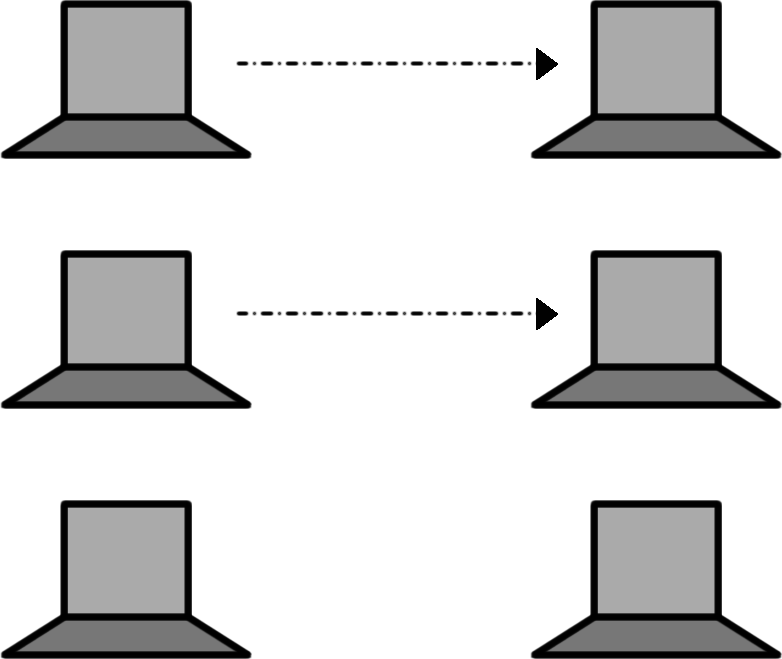
\includegraphics[width=0.5\linewidth]{mix_1-1.png}
%\captionof{figure}{Mixed point to point}\label{figtop:mix_1-1}
%\end{minipage}
%\begin{minipage}[!h]{0.5\textwidth}
%\centering
%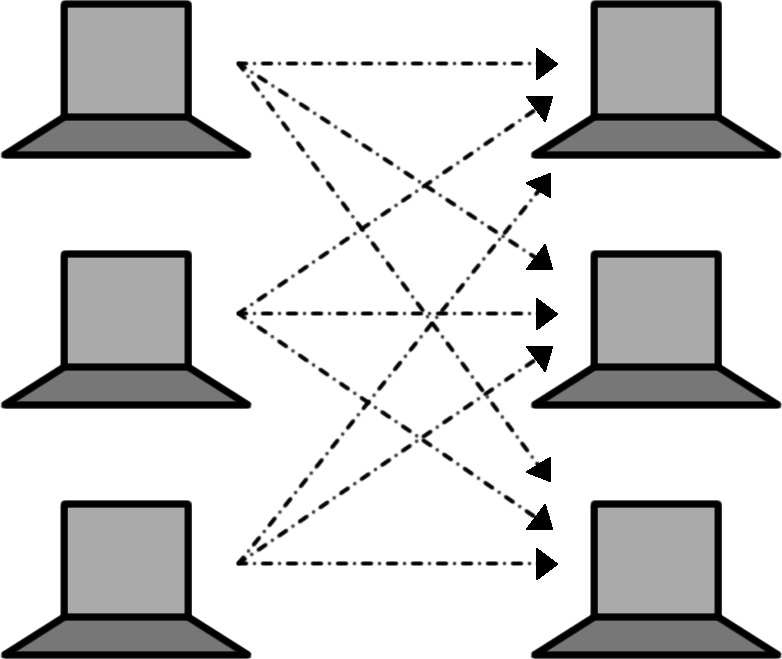
\includegraphics[width=0.5\linewidth]{1-N.png}
%\captionof{figure}{Bipartition}\label{figtop:1-n}
%\end{minipage}

%\begin{figure}[!h]
%  \begin{minipage}{0.5\textwidth}
%    \centering
%    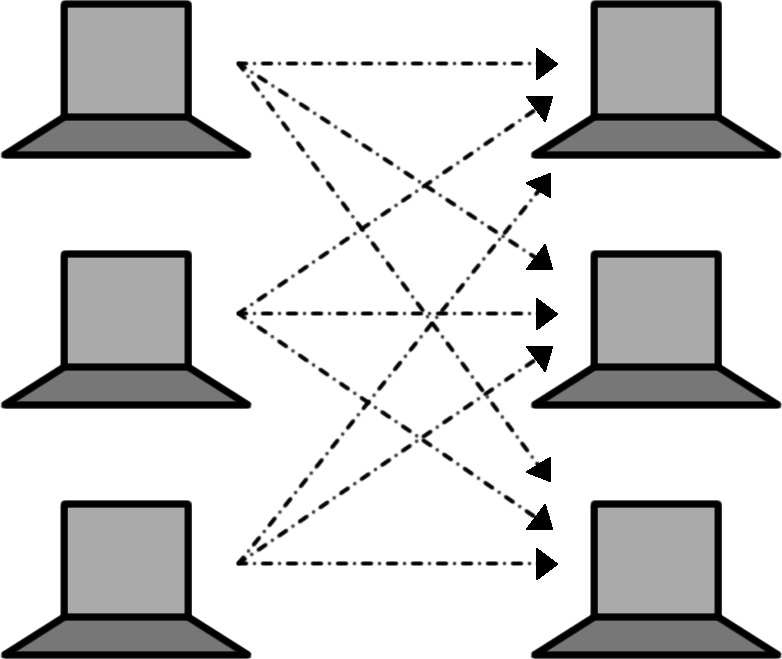
\includegraphics[width=0.5\textwidth{mix_1-1.png}
%    \caption{Mixed point to point}\label{figtop:mix_1-1}
%  \end{minipage}
%  \hfill
%  \begin{minipage}{0.5\textwidth}
%  \centering
%    \includegraphics[width=0.5\textwidth]{1-N.png}
%    \caption{Bipartition}\label{figtop:1-n}
%  \end{minipage}
%\end{figure}
\begin{figure}[!h]
  \begin{minipage}[b]{0.5\textwidth}
    \centering
    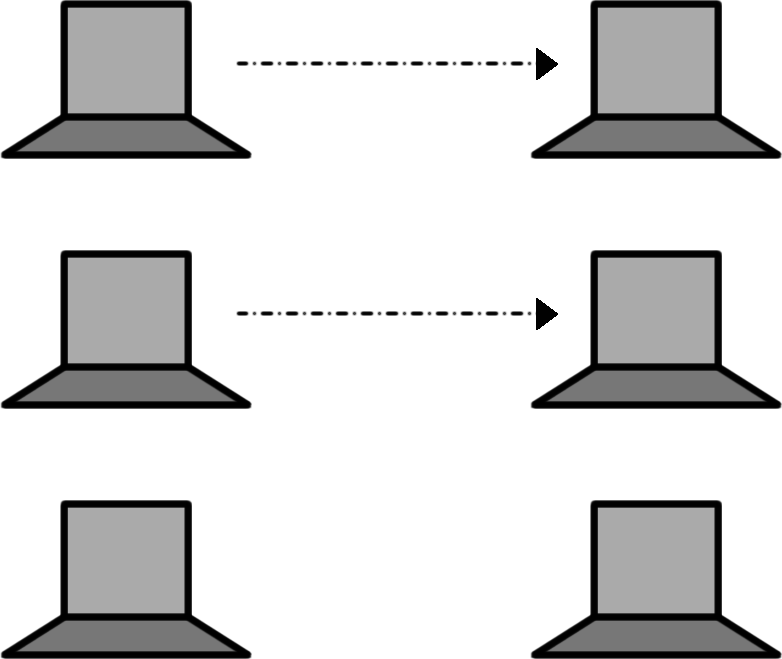
\includegraphics[width=0.6\textwidth]{mix_1-1.png}
    \caption{Mixed point to point}\label{figtop:mix_1-1}
  \end{minipage}
  \hfill
  \begin{minipage}[b]{0.5\textwidth}
  \centering
    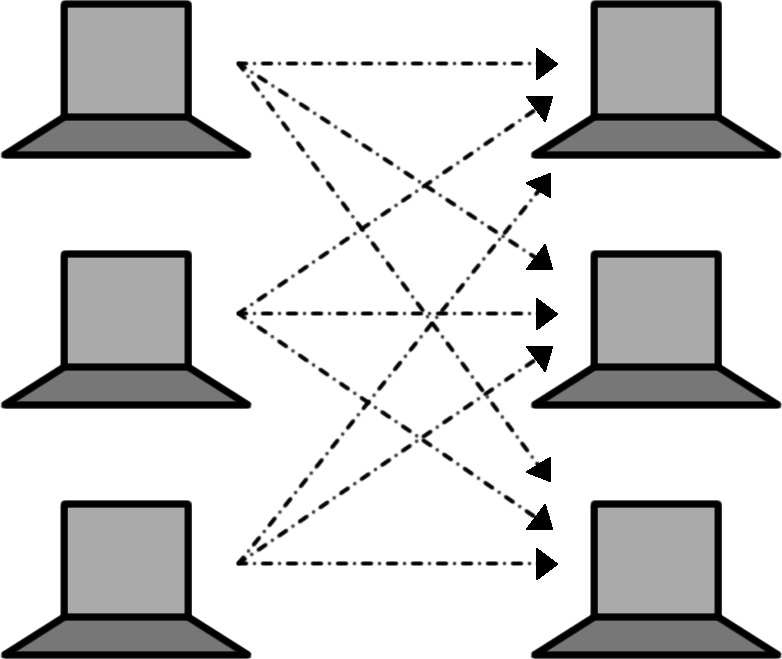
\includegraphics[width=0.6\textwidth]{1-N.png}
    \caption{Bipartition}\label{figtop:1-n}
  \end{minipage}
\end{figure}



%\begin{minipage}[!h]{0.5\textwidth}
%\centering
%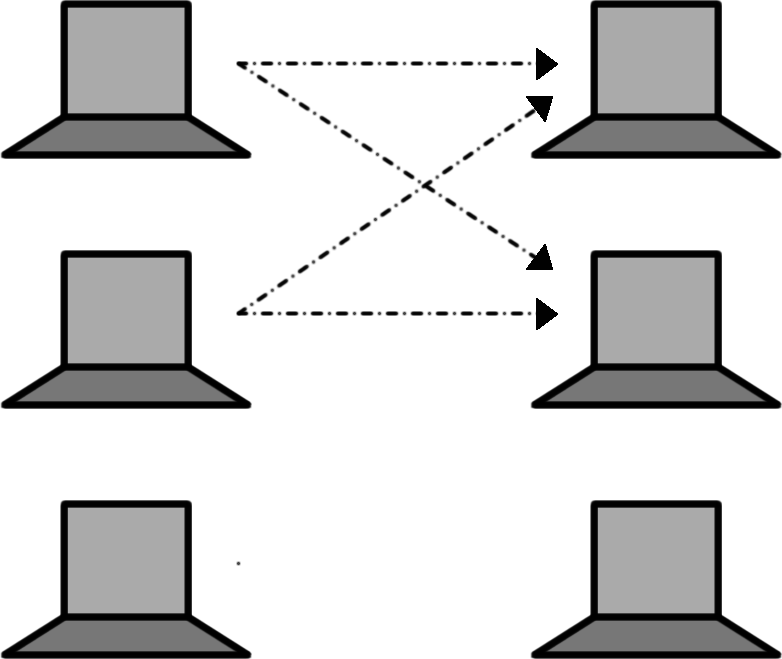
\includegraphics[width=0.5\linewidth]{mix_1-N.png}
%\captionof{figure}{Mixed bipartition}\label{figtop:mix_1-n}
%\end{minipage}
%\begin{minipage}[!h]{0.5\textwidth}
%\centering
%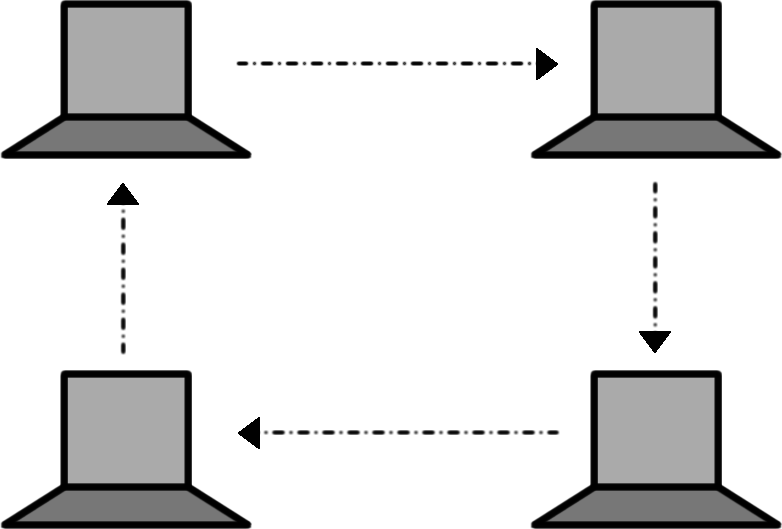
\includegraphics[width=0.5\linewidth]{top_cyc.png}
%\captionof{figure}{Ring}\label{figtop:cyc}
%\end{minipage}

\begin{table}[!h]
\centering
\renewcommand{\arraystretch}{1}
\begin{tabular}[t]{|p{3.5cm}|p{10.5cm}|}
	\hline
	\textbf{Strategy name} & {\sc Simple communication strategy} (variant B)\\
	\hline
	\textbf{Cooperative} & 
	\begin{tabular}[t]{@{}l@{}}
	$\text{\rlap{$\checkmark$}}\square$ Yes\\
	$\square$ No
	\end{tabular}\\
	\hline
	\textbf{Description} & Same solver structure in the \soset{}. Communication in one sense of the current configuration, performed while applying the \textit{reset}.\\
	\hline
	\textbf{Topologies} &
	\begin{tabular}[t]{@{}l@{}}
	$\vardiamond$ Point to point \\
	$\vardiamond$ Bipartition \\
	\end{tabular}\\
	\hline
	{\bf Benchmarks} & 
	\begin{tabular}[t]{@{}l@{}}
		\carrp\\
	\end{tabular}\\
	\hline
\end{tabular}
\label{tab_resume:simpleB}
\end{table}

\begin{figure}[!h]
  \begin{minipage}[b]{0.5\textwidth}
    \centering
    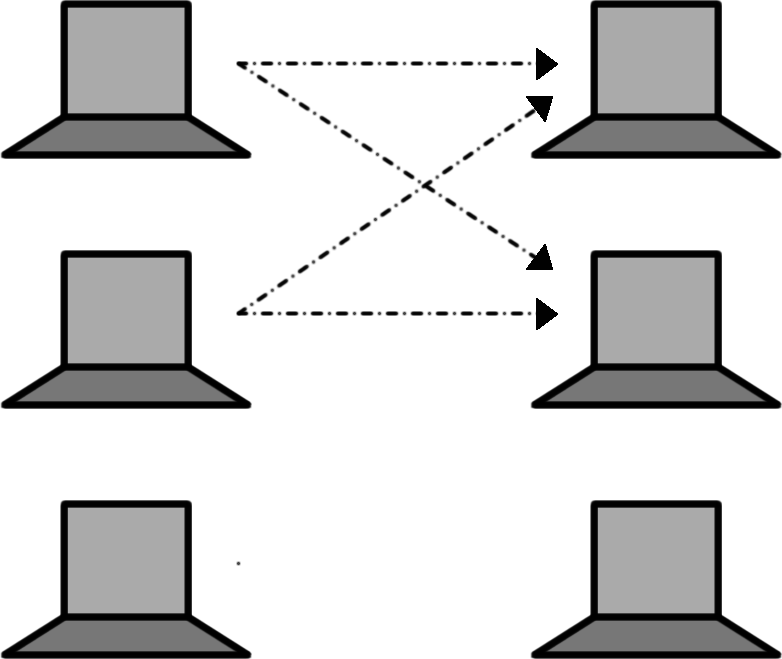
\includegraphics[width=0.6\textwidth]{mix_1-N.png}
    \caption{Mixed bipartition}\label{figtop:mix_1-n}
  \end{minipage}
  \hfill
  \begin{minipage}[b]{0.5\textwidth}
  \centering
    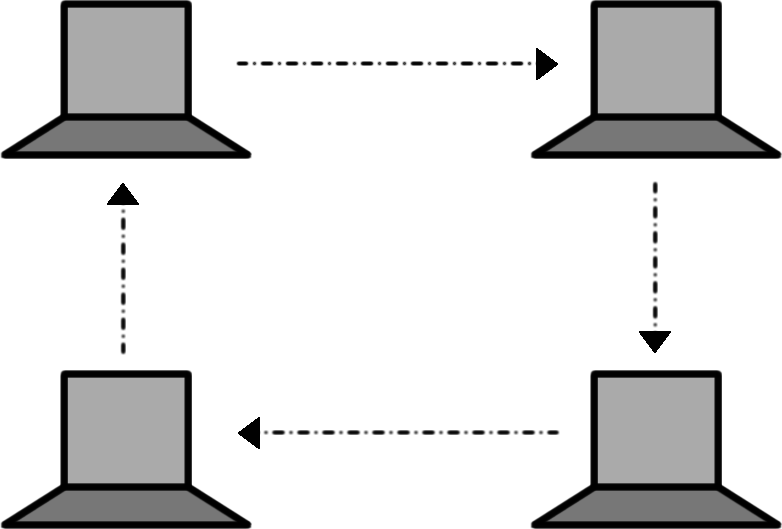
\includegraphics[width=0.6\textwidth]{top_cyc.png}
    \caption{Ring}\label{figtop:cyc}
  \end{minipage}
\end{figure}

%\begin{minipage}{0.5\textwidth}
%\centering
%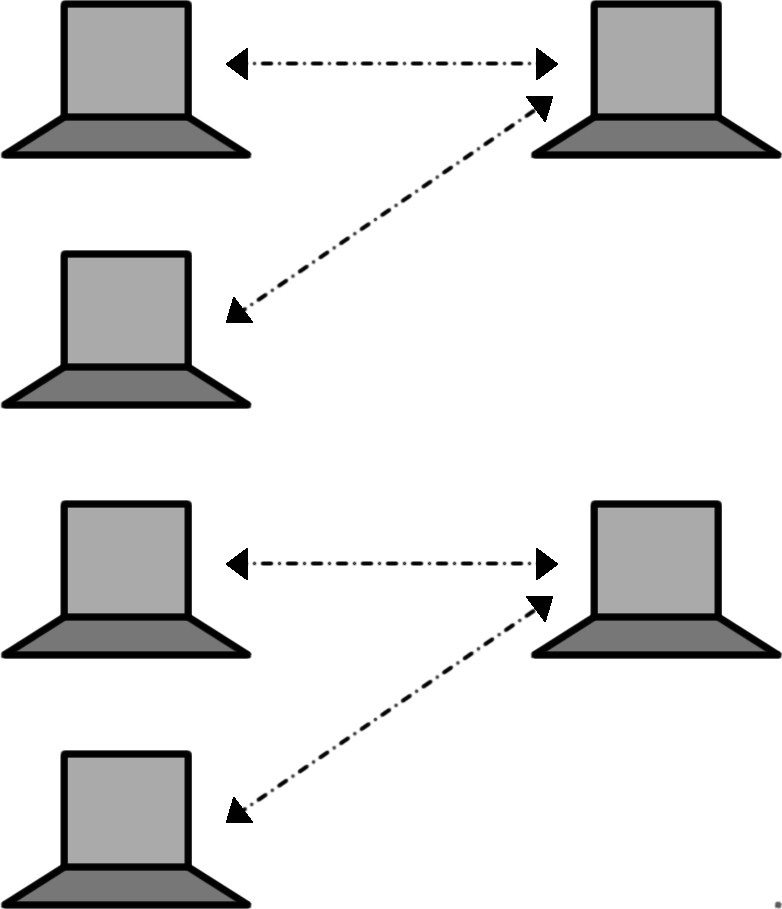
\includegraphics[width=0.5\linewidth]{2S_N-1.png}
%\captionof{figure}{Cyclic bipartition by groups}\label{figtop:2s_bip}
%\end{minipage}
%\begin{minipage}{0.5\textwidth}
%\centering
%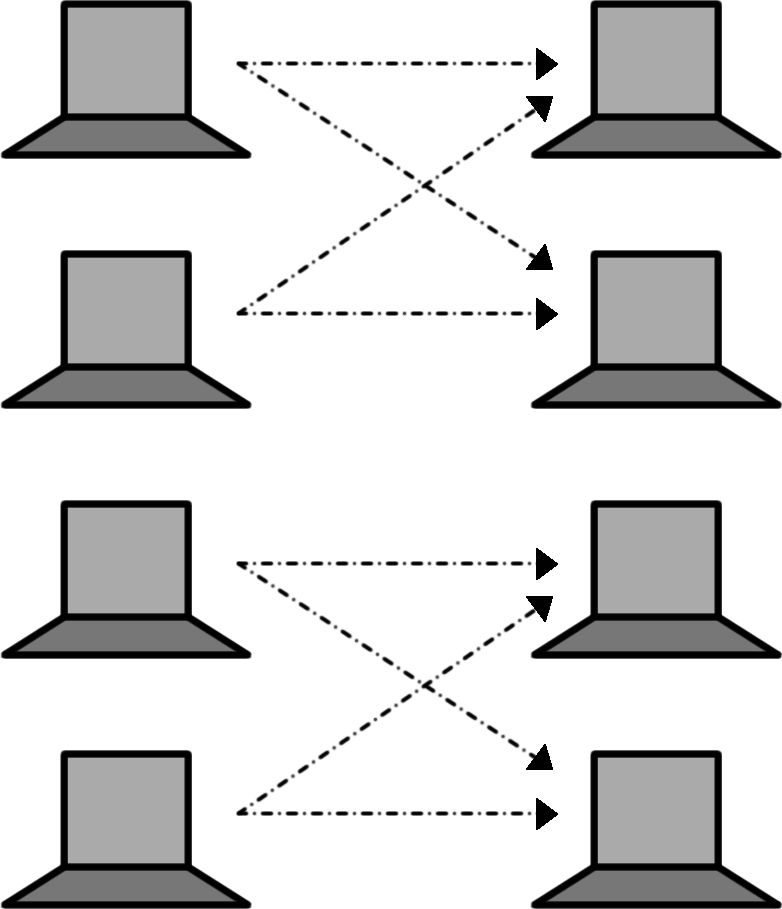
\includegraphics[width=0.5\linewidth]{group_1-N.png}
%\captionof{figure}{Bipartition by groups}\label{figtop:gr_bip}
%\end{minipage}

\begin{table}[!h]
\centering
\renewcommand{\arraystretch}{1}
\begin{tabular}[t]{|p{3.5cm}|p{10.5cm}|}	
	\hline
	\textbf{Strategy name} & {\sc Circular exchange}\\
	\hline
	\textbf{Cooperative} & 
	\begin{tabular}[t]{@{}l@{}}
	$\text{\rlap{$\checkmark$}}\square$ Yes\\
	$\square$ No
	\end{tabular}\\
	\hline
	\textbf{Description} & Circular communication of the current configuration, performed while applying the acceptance criterion of the new configuration for the next iteration. In each iteration a solver obtains a new derived configurations by modifying a portion of the received configuration. Information exchange takes place after a certain number of iterations. \\
	\hline
	\textbf{Topology} & 
	\begin{tabular}[t]{@{}l@{}}
	$\vardiamond$ Ring (See Figure~\ref{figtop:cyc})
	\end{tabular}\\
	\hline
	{\bf Benchmarks} & 
	\begin{tabular}[t]{@{}l@{}}
		\sgp\\
	\end{tabular}\\
	\hline
\end{tabular}
\label{tab_resume:circular}
\end{table}

\begin{figure}[!h]
  \begin{minipage}[b]{0.5\textwidth}
    \centering
    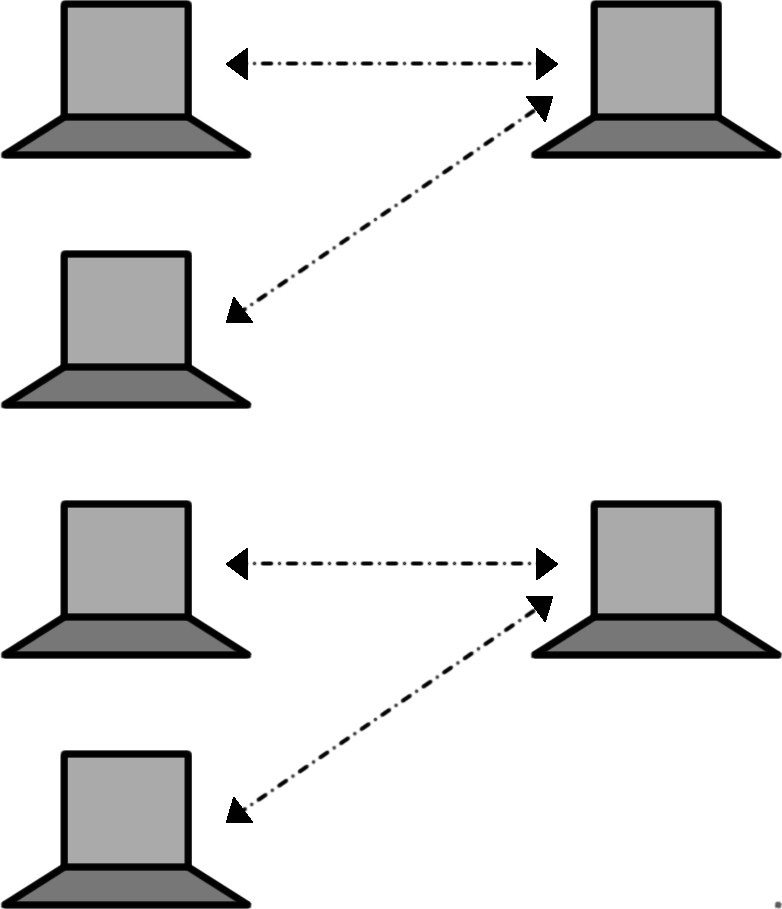
\includegraphics[width=0.6\textwidth]{2S_N-1.png}
    \caption{Cyclic bipartition by groups}\label{figtop:2s_bip}
  \end{minipage}
  \hfill
  \begin{minipage}[b]{0.5\textwidth}
  \centering
    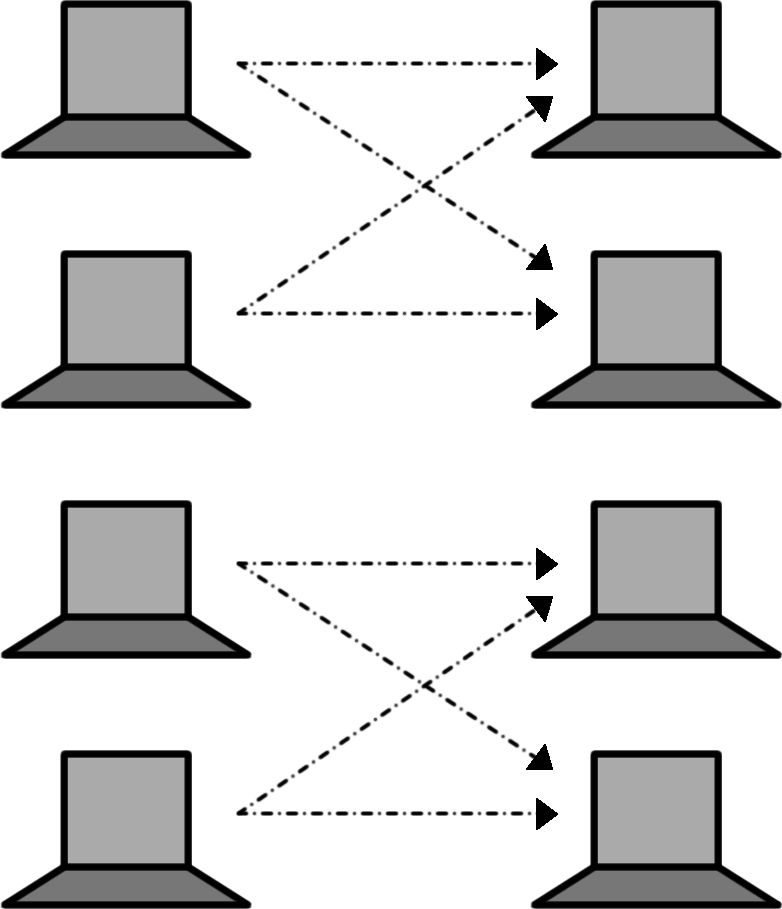
\includegraphics[width=0.6\textwidth]{group_1-N.png}
    \caption{Bipartition by groups}\label{figtop:gr_bip}
  \end{minipage}
\end{figure}


\begin{table}[!h]
\centering
\renewcommand{\arraystretch}{1}
\begin{tabular}[t]{|p{3.5cm}|p{10.5cm}|}
	\hline
	\textbf{Strategy name} & {\sc Companion-standard exchange}\\
	\hline
	\textbf{Cooperative} & 
	\begin{tabular}[t]{@{}l@{}}
	$\text{\rlap{$\checkmark$}}\square$ Yes\\
	$\square$ No
	\end{tabular}\\
	\hline
	\textbf{Description} & Communication of the current configuration, performed while applying the acceptance criterion of the new configuration for the next iteration.\\
	\hline
	\textbf{Topology} & 
	\begin{tabular}[t]{@{}l@{}}
	$\vardiamond$ Cyclic point to point (See Figure~\ref{figtop:cyc_1-1})\\
	$\vardiamond$ Mixed cyclic point to point (See Figure~\ref{figtop:mix_cyc_1-1})\\
	$\vardiamond$ Cyclic bipartition by groups \\
	\end{tabular}\\
	\hline
	{\bf Benchmarks} & 
	\begin{tabular}[t]{@{}l@{}}
		\sgp{} \\ \nqp{} 
	\end{tabular}\\
	\hline
\end{tabular}
%\caption{\sgp}
\label{tab_resume:sgp_good}
\end{table}

\begin{figure}[!h]
  \begin{minipage}[b]{0.5\textwidth}
    \centering
    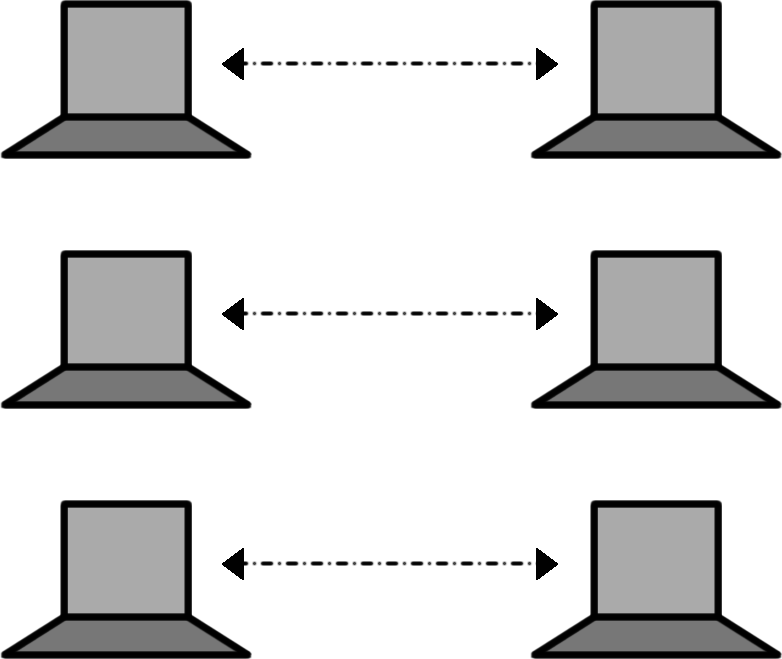
\includegraphics[width=0.6\textwidth]{2S_1-1.png}
    \caption{Cyclic point to point}\label{figtop:cyc_1-1}
  \end{minipage}
  \hfill
  \begin{minipage}[b]{0.5\textwidth}
  \centering
    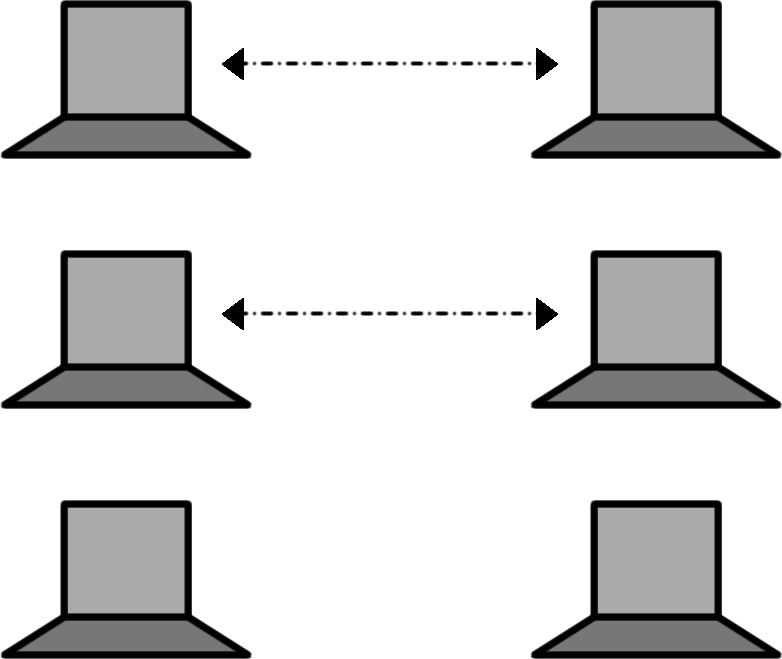
\includegraphics[width=0.6\textwidth]{mix_2S_1-1.png}
        \caption{Mixed cyclic point to point}\label{figtop:mix_cyc_1-1}
  \end{minipage}
\end{figure}

%\begin{figure}[!h]
%\centering
%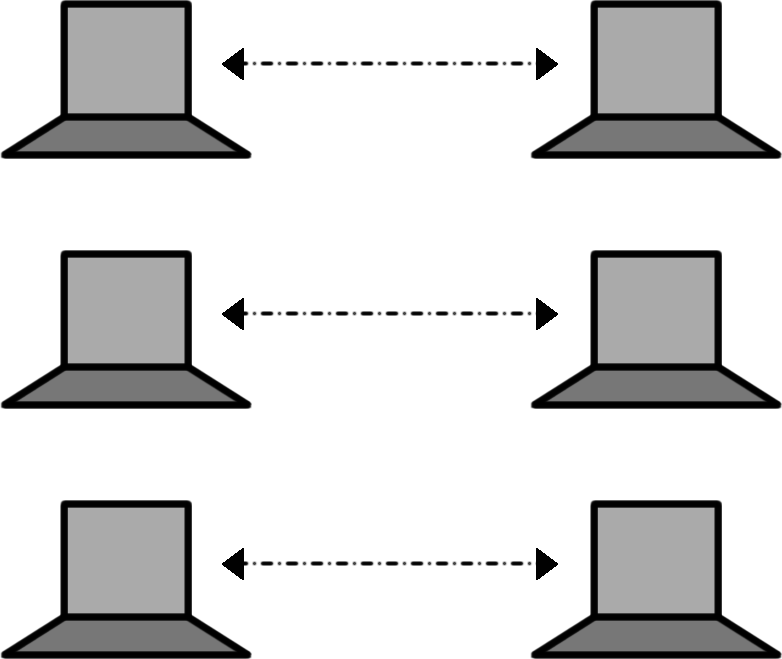
\includegraphics[width=0.25\linewidth]{2S_1-1.png}
%\caption{Cyclic point to point}\label{figtop:cyc_1-1}
%\end{figure}


\begin{table}[!h]
\centering
\renewcommand{\arraystretch}{1}
\begin{tabular}[t]{|p{3.5cm}|p{10.5cm}|}
	\hline
	\textbf{Strategy name} & {\sc Local minima evasion}\\
	\hline
	\textbf{Cooperative} & 
	\begin{tabular}[t]{@{}l@{}}
	$\text{\rlap{$\checkmark$}}\square$ Yes\\
	$\square$ No
	\end{tabular}\\
	\hline
	\textbf{Description} & Same solver structure in the \soset{}. Communication in one sense of the current configuration, performed by the sender when this current configuration is classified as a local minima (after a number of iterations without improving the current cost), and by the receiver while performing the restart.\\
	\hline
	\textbf{Topologies} &
	\begin{tabular}[t]{@{}l@{}}
	$\vardiamond$ Point to point \\
	$\vardiamond$ Bipartition \\
	\end{tabular}\\
	\hline
	{\bf Benchmarks} & 
	\begin{tabular}[t]{@{}l@{}}
		\grp\\
	\end{tabular}\\
	\hline	
\end{tabular}
%\caption{\sgp}
\label{tab_resume:grp_comm}
\end{table}